\chapter{Implementation}
\label{chap:Implementation}

\section{Broker Implementation}
\label{sec:Broker Implementation}

\todo[inline]{High level overview of the broker architecture (blocks/channels/message flows etc.), as well as datastructures/algorithms used}

\subsection{Connection Manager}
\label{sub:Connection Manager}

\todo[inline]{Overview of the connection manager (TCP/UDP connections etc.)}

\subsection{Message Storage}
\label{sub:Message Handlers}

In the event that, for whatever reason, a client is not ready to accept a
message when it arrives - this message must be buffered up in a datastructure of
some kind, until delivery is possible. There are a number of different
datastructures that could be used - each with its own pros and cons. \\

As mentioned in Section~\ref{sub:pubsub}, message brokers typically support a
number of different delivery patterns, the two most common of which are Queues
(Section~\ref{sub:queues}) and Topics (Section~\ref{sub:topics}). The backing
datastructures used for each are explored below. \\

Queues require that messages are delivered in the order they are pushed onto the
queue, and that each message is delivered to a single consumer - so any backing
datastructure must support this. Queues typically support two main operations:

\begin{description}
  \item[\textit{enqueue(m)}] \hfill \\
    The message $m$ is placed onto the queue.
  \item[\textit{dequeue()}] \hfill \\
    Returns the message at the front of the queue (optionally blocks whilst the queue is empty)
\end{description}

The simplest method of representing a queue of messages, would be an array. New
messages are inserted into the first unoccupied slot in the array, and messages
are read front-to-back, in a \gls{fifo} fashion.

\begin{figure}[H]
  \centering
  \begin{subfigure}[b]{\textwidth}
    \centering
    \begin{tikzpicture}

\coordinate (s) at (0,0);
\foreach \num in {0,...,6}{
    \ifthenelse{\num < 4}
    {\node[draw, minimum size=1cm] at (s) (\num) {m\num};} % Fill the box
    {\node[draw, minimum size=1cm] at (s) (\num) {};} % Don't fill the box

    \coordinate (s) at ($(s) + (1,0)$);
}

\node[above=1mm of 0] {$h$};
\node[above=1mm of 4] {$t$};

\end{tikzpicture}

    \caption{Messages are read from the head of the queue ($h$)}
    \label{fig:tikz:queueArrayInitial}
  \end{subfigure}

  \begin{subfigure}[b]{\textwidth}
    \centering
    \begin{tikzpicture}

\coordinate (s) at (0,0);
\foreach \num in {0,...,6}{
    \ifthenelse{\num > 0 \AND \num < 4}
    {\node[draw, minimum size=1cm] at (s) (\num) {m\num};} % Fill the box
    {\node[draw, minimum size=1cm] at (s) (\num) {};} % Don't fill the box

    \coordinate (s) at ($(s) + (1,0)$);
}

\node[above=1mm of 0] {$h$};
\node[above=1mm of 4] {$t$};

\end{tikzpicture}

    \caption{The array is shuffled down}
    \label{fig:tikz:queueArrayHeadRead}
  \end{subfigure}

  \begin{subfigure}[b]{\textwidth}
    \centering
    \begin{tikzpicture}

\coordinate (s) at (0,0);
\foreach \num in {1,...,7}{
    \ifthenelse{\num < 4}
    {\node[draw, minimum size=1cm] at (s) (\num) {m\num};} % Fill the box
    {\node[draw, minimum size=1cm] at (s) (\num) {};} % Don't fill the box

    \coordinate (s) at ($(s) + (1,0)$);
}

\node[above=1mm of 1] {$h$};
\node[above=1mm of 4] {$t$};

\end{tikzpicture}

    \caption{The next message is now ready to be read}
    \label{fig:tikz:queueArrayPostShuffle}
  \end{subfigure}
  \caption{Reading a message from an array-based queue}
  \label{fig:tikz:queueArray}
\end{figure}

However, there are several disadvantages of this approach, for both the enqueue and dequeue operations.

\begin{description}
  \item[\textit{enqueue(m)}] \hfill \\
    Arrays in GoLang have a fixed length - but there is no limit on the number
    of messages a queue may be asked to buffer. We can compensate for this by
    using 'slices' instead of arrays\todo{Explain slices - seperate section} -
    which are expandable using the \mintinline{go}{append()} command
    (Listing~\ref{lst:golangAppendToSlice}). The message $m$ is stored into the
    first available array index, which will typically complete in $O(1)$ time.
    However, in order to create the illusion of an 'expandable' array, slices
    use a fixed-length array under the hood - which is expanded when full. This
    expansion involves creating a new array, which is twice the size of the
    original. Each message in the underlying array is then copied to the new
    array, which is used for all slice actions going forward. Therefore, whilst
    the vast majority of messages will be stored in $O(1)$ time, a message that
    triggers an expansion of the underlying array will require $O(n)$ time to
    store (where $n$ is the number of messages in the queue)\todo{Improve
    notation}.
  \item[\textit{dequeue()}] \hfill \\
    Pulling the first message in the array requires that the array be shuffled
    after each \mintinline{go}{dequeue()} operation, so that the next message to
    be delivered always resides in  array position 0 (see in
    Figure~\ref{fig:tikz:queueArray}). An array implementation would be
    extremely inefficient, requiring $n - 1$ items to moved down an array
    position. However, because a slice is simply a 'view' onto an array, this
    operation can be made extremely efficient - by simply creating a new slice,
    with all but the first element in common with the original.\todo{Diagram?}
    It is therefore possible to complete this operation in $O(1)$ time.
\end{description}

\begin{listing}[H]
  \centering
  \inputminted[firstline=7, lastline=12]{go}{code/snippets/appendToSlice.go}
  \caption{An example of appending to a GoLang slice}
  \label{lst:golangAppendToSlice}
\end{listing}

In addition to the disadvantages given above, slices are quite inefficient when
it comes to memory utilisation. At any moment in time, up to 50\% of the
underlying array will be empty. Whilst these array indexes do not contain
messages, they still occupy space in memory, meaning that (in the worst case
scenario) $O(2n)$ space is required to store $n$ messages. This is not ideal.

An alternative method of representing an in-memory-queue, is a linked list
(Figure~\ref{fig:tikz:queueLinkedList}). This has numerous advantages over an
array - with both enqueue and dequeue operations completing in $O(1)$ time.
Linked lists also improve on the space complexity of the queue, as the
datastructure grows and shrinks in response  to the number of messages - meaning
that we require $O(n)$ memory to store $n$ messages.

\begin{description}
  \item[\textit{enqueue(m)}] \hfill \\
    The item at the tail of the queue ($t$) - seen in
    Figure~\ref{fig:tikz:queueLinkedListInitial} - is simply updated with a
    pointer to $m$. This is an $O(1)$ operation, and simple to perform.
  \item[\textit{dequeue()}] \hfill \\
    The item at the head of the queue ($h$) is returned. The head pointer is
    then updated to point to the next message to be read, as in
    Figure~\ref{fig:tikz:queueLinkedListHeadRead}.
\end{description}

\begin{figure}[H]
  \centering
  \begin{subfigure}[b]{\textwidth}
    \centering
    \begin{tikzpicture}[thick]

\coordinate (s) at (0,0);
\foreach \num[remember=\num as \previous] in {0,...,4}{
    \node[draw, minimum size=1cm] at (s) (\num) {m\num};

    \ifthenelse{\num > 0}
    {\draw[->](\previous) edge (\num);}
    {}

    \coordinate (s) at ($(s) + (2,0)$);
}


\node[above=0.5cm of 0] (head) {$h$};
\node[above=1mm of 4] {$t$};
\draw[->,thick](head) edge (0);

\end{tikzpicture}

    \caption{Messages are read from the head of the queue ($h$)}
    \label{fig:tikz:queueLinkedListInitial}
  \end{subfigure}

  \begin{subfigure}[b]{\textwidth}
    \centering
    \begin{tikzpicture}[thick]

\coordinate (s) at (0,0);
\foreach \num[remember=\num as \previous] in {0,...,4}{
    \ifthenelse{\num < 2}
    {\node[draw, minimum size=1cm, gray] at (s) (\num) {m\num};}
    {\node[draw, minimum size=1cm] at (s) (\num) {m\num};}

    \ifthenelse{\num < 3}
    {\ifthenelse{\num > 0}{\draw[->, gray](\previous) edge (\num);}{}}
    {\draw[->](\previous) edge (\num);}

    \coordinate (s) at ($(s) + (2,0)$);
}


\node[above=0.5cm of 2] (head) {$h$};
\node[above=1mm of 4] {$t$};
\draw[->](head) edge (2);

\end{tikzpicture}

    \caption{Head moves, and read nodes are marked for garbage collection}
    \label{fig:tikz:queueLinkedListHeadRead}
  \end{subfigure}

  \begin{subfigure}[b]{\textwidth}
    \centering
    \begin{tikzpicture}[thick]

\coordinate (s) at (0,0);
\foreach \num[remember=\num as \previous] in {0,...,4}{
    \ifthenelse{\num < 2}
    { % These have been garbage collected
      \node[draw, minimum size=1cm, gray] at (s) (\num) {m\num};
      \node(Cross) [draw,cross out,minimum width=1cm,minimum height=1cm,red] at (s) {};
    }
    { % These are still active
      \node[draw, minimum size=1cm] at (s) (\num) {m\num};
    }

    % Don't draw 'next' pointers for dead nodes
    \ifthenelse{\num > 2}{\draw[->](\previous) edge (\num);}{}

    \coordinate (s) at ($(s) + (2,0)$);
}

\node[above=0.5cm of 2] (head) {$h$};
\node[above=1mm of 4] {$t$};
\draw[->](head) edge (2);

\end{tikzpicture}

    \caption{At some point in the future (depending on memory pressure), the
             \gls{gc} will automatically clean up the read messages}
    \label{fig:tikz:queueLinkedListGCRun}
  \end{subfigure}
  \caption{Reading a message from an array-based queue}
  \label{fig:tikz:queueLinkedList}
\end{figure}

A full implementation of a linked list queue can be found in
Appendix~\ref{appendix:queueCode}.

When it comes to representing topics, the situation is similar. As mentioned in
Section~\ref{sub:topics}, the main difference between queues and topics, is the
fact that queues deliver each message to a single consumer, whereas topics
deliver each message to \emph{all} consumers. This requires a subtly different
datastructure to hold the messages - as consumers may read messages at different
rates.\todo{Figure} If we use an array-based datastructure, similar to that in
Figure~\ref{fig:tikz:queueArray}, we would be required to maintain a seperate
queue for each subscriber\todo{Figure} to read from. A topic with $s$
subscribers, and $n$ pending messages would therefore require at \emph{least}
$O(n * s)$ memory, and that is without considering the caveats described
above\todo{XReference}. \\

A linked-list implementation, however, has the potential to be highly efficient
when it comes to storage space. Rather than storing $s$ messages, we can simply
keep multiple 'head' pointers on the same linked-list, one for each subscriber.
When a subscriber consumes a message - only the head pointer belonging to it is
moved up the list, the rest remain static. This method only requires $O(s + m)$
memory, for a topic with $s$ subscribers, and $m$ messages. The linked-list
implementation of a topic therefore has an even bigger efficiency saving over
the corresponding array-based implementation, than in the queue examples given
above, as seen in Figure~\ref{fig:tikz:implementationSpaceComplexityGraph}.

\begin{figure}[H]
  \centering
  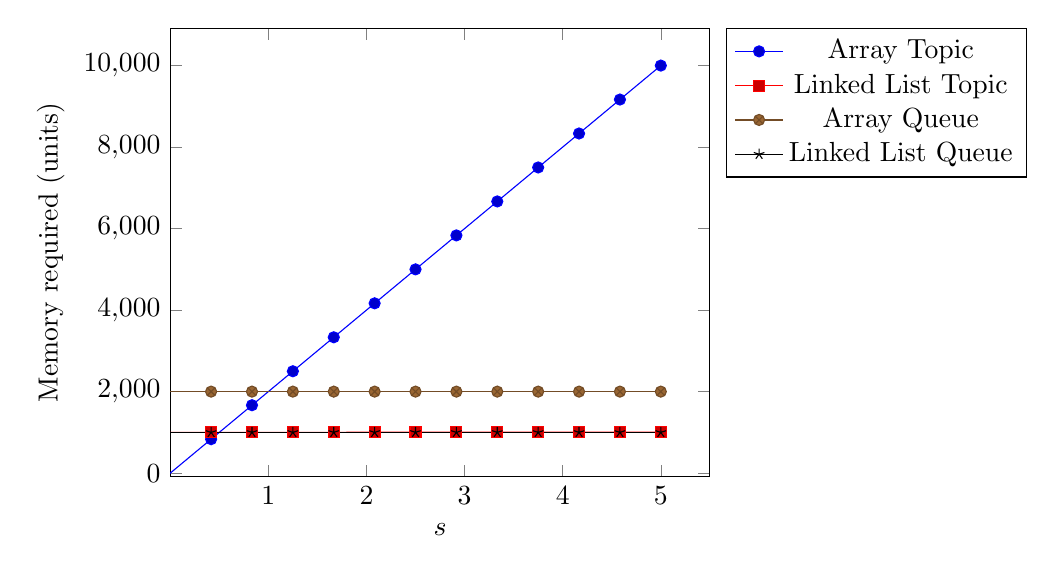
\begin{tikzpicture}
\begin{axis}[
    xlabel=$s$,
    ylabel={Memory required (units)},
    xmin=0,
    xtick={1,...,10},
    scaled ticks=false,
    legend entries={Array Topic, Linked List Topic, Array Queue, Linked List Queue},
    legend pos=outer north east,
]
\addplot {2 * x * 1000};
\addplot {x + 1000};
\addplot {2 * 1000};
\addplot {1000};
\end{axis}
\end{tikzpicture}

  \caption{A comparison of the space complexities of various queue/topic
           implementations, as the number of subscribers ($s$) increases}
  \label{fig:tikz:implementationSpaceComplexityGraph}
\end{figure}

\subsection{Message Shipper}
\label{sub:Message Shipper}

\todo[inline]{Message delivery/queue/topic behavior}

\subsection{Metrics Manager}
\label{sub:Metrics Manager}

\todo[inline]{Metric format/serialization. How do we ensure minimal CPU usage}

\section{Presentation Interface}
\label{sec:Presentation Interface}

\todo[inline]{Screenshots/high-level description}

\subsection{Graphite/Grafana}
\label{sub:Graphite/Grafana}

\todo[inline]{Architecture}

\subsection{Docker}
\label{sub:Docker}

\todo[inline]{Overview and Dockerfile description}

\section{Utilities}
\label{sec:Utilities}

\todo[inline]{Python benchmark code walkthrough}

\subsection{Configuration}
\label{sub:Configuration}

\todo[inline]{Specifics of command-line flag/config file implementation}
